% This must be in the first 5 lines to tell arXiv to use pdfLaTeX, which is strongly recommended.
\pdfoutput=1
% In particular, the hyperref package requires pdfLaTeX in order to break URLs across lines.

\documentclass[11pt]{article}
%\usepackage[toc]{appendix}
% Remove the "review" option to generate the final version.
\usepackage[review]{acl}

% Standard package includes
\usepackage{times}
\usepackage{latexsym}
\usepackage{graphicx}
% For proper rendering and hyphenation of words containing Latin characters (including in bib files)
\usepackage[T1]{fontenc}
% For Vietnamese characters
% \usepackage[T5]{fontenc}
% See https://www.latex-project.org/help/documentation/encguide.pdf for other character sets

% This assumes your files are encoded as UTF8
\usepackage[utf8]{inputenc}

% This is not strictly necessary, and may be commented out,
% but it will improve the layout of the manuscript,
% and will typically save some space.
\usepackage{microtype}

% If the title and author information does not fit in the area allocated, uncomment the following
%
\setlength\titlebox{5cm}
%
% and set <dim> to something 5cm or larger.

\title{Logically at the Constraint 2022: Multimodal role labelling}

% Author information can be set in various styles:
% For several authors from the same institution:
% \author{Ludovic Kun *,\authormark{1} Jayesh Bankoti *,\authormark{1} and David Kiskovski\authormark{1}}
% \author[1,2,3]{Author One}
% \author[2,*]{Author Two}
% \author[1]{Author Three}

% \affil[1]{Publications Department, Optica Publishing Group, 2010 Massachusetts Avenue NW, Washington DC} 
%
\author{Ludovic Kun * , Jayesh Bankoti * , \and David Kiskovski \\ Logically, London, UK}
% \affil[*]{Corresponding author: email@my-email.com}
% if the names do not fit well on one line use
%         Author 1 \\ {\bf Author 2} \\ ... \\ {\bf Author n} \\
% For authors from different institutions:
% \author{Author 1 \\ Address line \\  ... \\ Address line
%         \And  ... \And
%         Author n \\ Address line \\ ... \\ Address line}
% To start a seperate ``row'' of authors use \AND, as in
% \author{Author 1 \\ Address line \\  ... \\ Address line
%         \AND
%         Author 2 \\ Address line \\ ... \\ Address line \And
%         Author 3 \\ Address line \\ ... \\ Address line}

%\author{First Author \\
%  Affiliation / Address line 1 \\
%  Affiliation / Address line 2 \\
%  Affiliation / Address line 3 \\
%  \texttt{email@domain} \\\And
%  Second Author \\
%  Affiliation / Address line 1 \\
%  Affiliation / Address line 2 \\
%  Affiliation / Address line 3 \\
%  \texttt{email@domain} \\}

\begin{document}
\maketitle
\begin{abstract}


This paper describes our system for the Constraint 2022 challenge at ACL 2022, whose goal is to detect which entities are glorified, vilified or victimised, within a meme . The task should be done considering the perspective of the meme's author. In our work, the challenge is treated
as a multi-class classification task. For a given pair of a meme and an entity, we need to classify whether the entity is being referenced as Hero, a Villain, a Victim or Other. 
Our solution combines (ensembling) different models based on Unimodal (Text only) model and Multimodal model (Text + Images). We conduct several experiments and benchmarks different competitive pre-trained
transformers and vision models in this work. Our solution, based on an ensembling method, is ranked first on the leaderboard and obtains a macro F1-score of 0.58 on test set. The code for the experiments and results are available at \href{https://bitbucket.org/logicallydevs/constraint_2022/src/master/}{here} .




\end{abstract}

\section{Introduction}

The rapid rise in the amount of harmful content being spread online is becoming a major societal challenge, with still unknown negative consequences. Large resources have been invested by many actors in the field of social media to shield users from harmful content. It is imperative to understand in a systematic way how information is spread, and be able to scalably monitor existing narratives and flag hateful ones circulating using technology. One way this is done is using entity recognition coupled with entity sentiment \cite{kiritchenko2021confronting}. The former technique is to support OSINT(open source intelligence) analysts in understanding who or what are the subjects of discussion, and the latter automates the process of analysing if they are coupled with positive or negative feelings, in order to assist with understanding the stance of online users on specific topics. Efforts to tackle this challenge were mainly focused on English-language text-based data formats such as articles \cite{wankhade2022survey}. However, the complexity of content being posted online has drastically increased over time, and the challenge of harmful content detection now extends to multimedia, including memes \cite{alam2021survey}. The emergence and proliferation of memes on social media have made their analysis a crucial challenge to understand online interactions. A point can also be made about the study of entities sentiment online, as the polarising portrayal of famous (or infamous) personalities or institutions often give rise to inflammatory views and content. 


Extracting insights from memes is a novel field and still has a lot of opportunities for growth. The multimodality of text and image adds a layer of complexity which contains more information, but is also harder to extract. Indeed each modality needs to understand their intrinsic properties but also capture cross-modal semantic understanding \cite{muller2021multimodal}. This paper delves into the field of multimodal semantic role labelling, a new task with particular challenges.

Examples of the multimodal dataset \cite{sharma2022report} used to tackle this problem and provided as part of the CONSTRAINT competition are presented in Figure ~\ref{fig:Constraint dataset examples}. The first sample shows a meme image displaying two politicians from opposite parties separated on two sides of the image, with text around them, as well as the associated JSON line input with the extracted text from the image (also known as Optical Character Recognition or OCR), as well as the entities' mentioned labelled roles. In this case, all entities are referenced in the text of the image. In the second sample, however, we notice that not all are mentioned in the text, and visual information is needed to classify all entities.
\begin{figure}
\centering
    %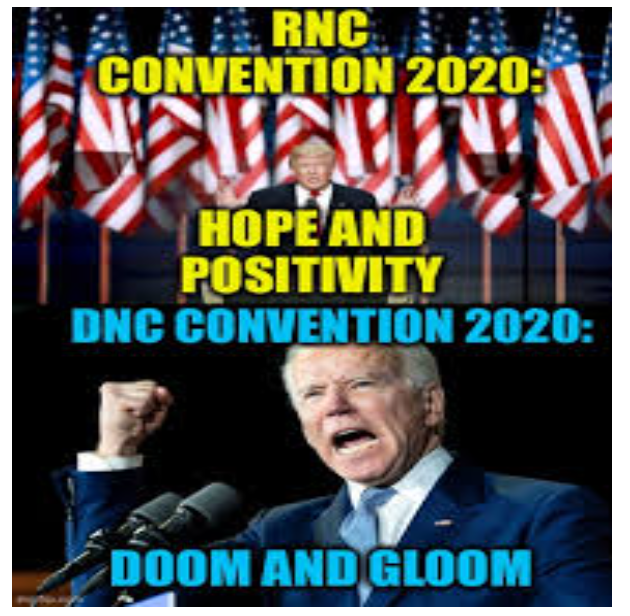
\includegraphics[scale=0.6]{exampleconstraint.PNG}
    %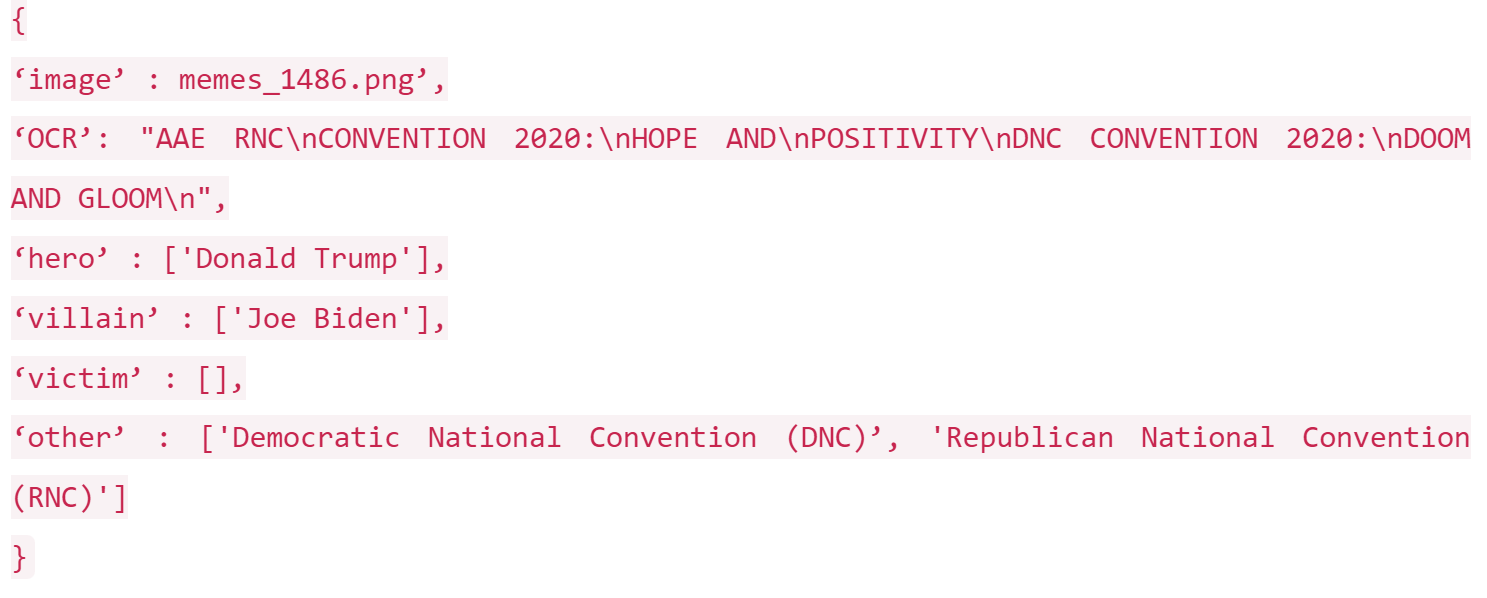
\includegraphics[scale=0.3]{constraint.PNG}
    %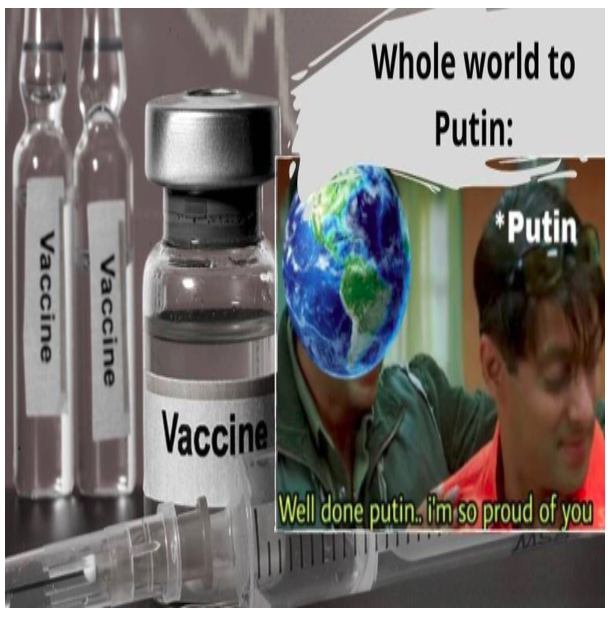
\includegraphics[scale=0.60]{2.PNG}
    %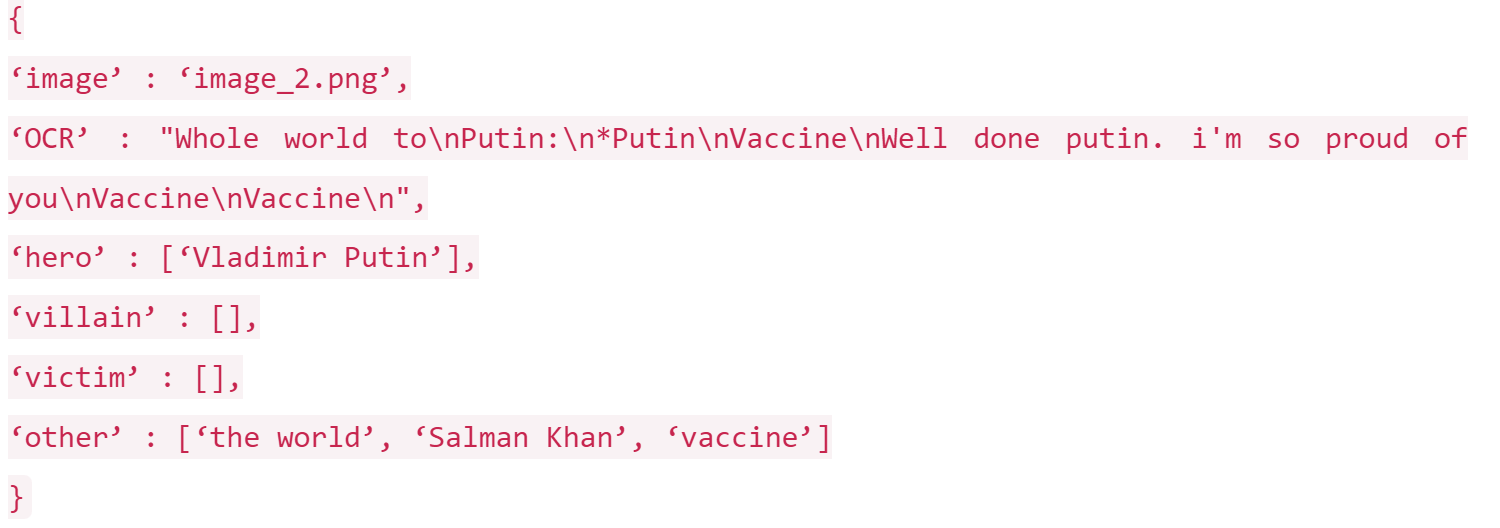
\includegraphics[scale=0.3]{2json.PNG}
    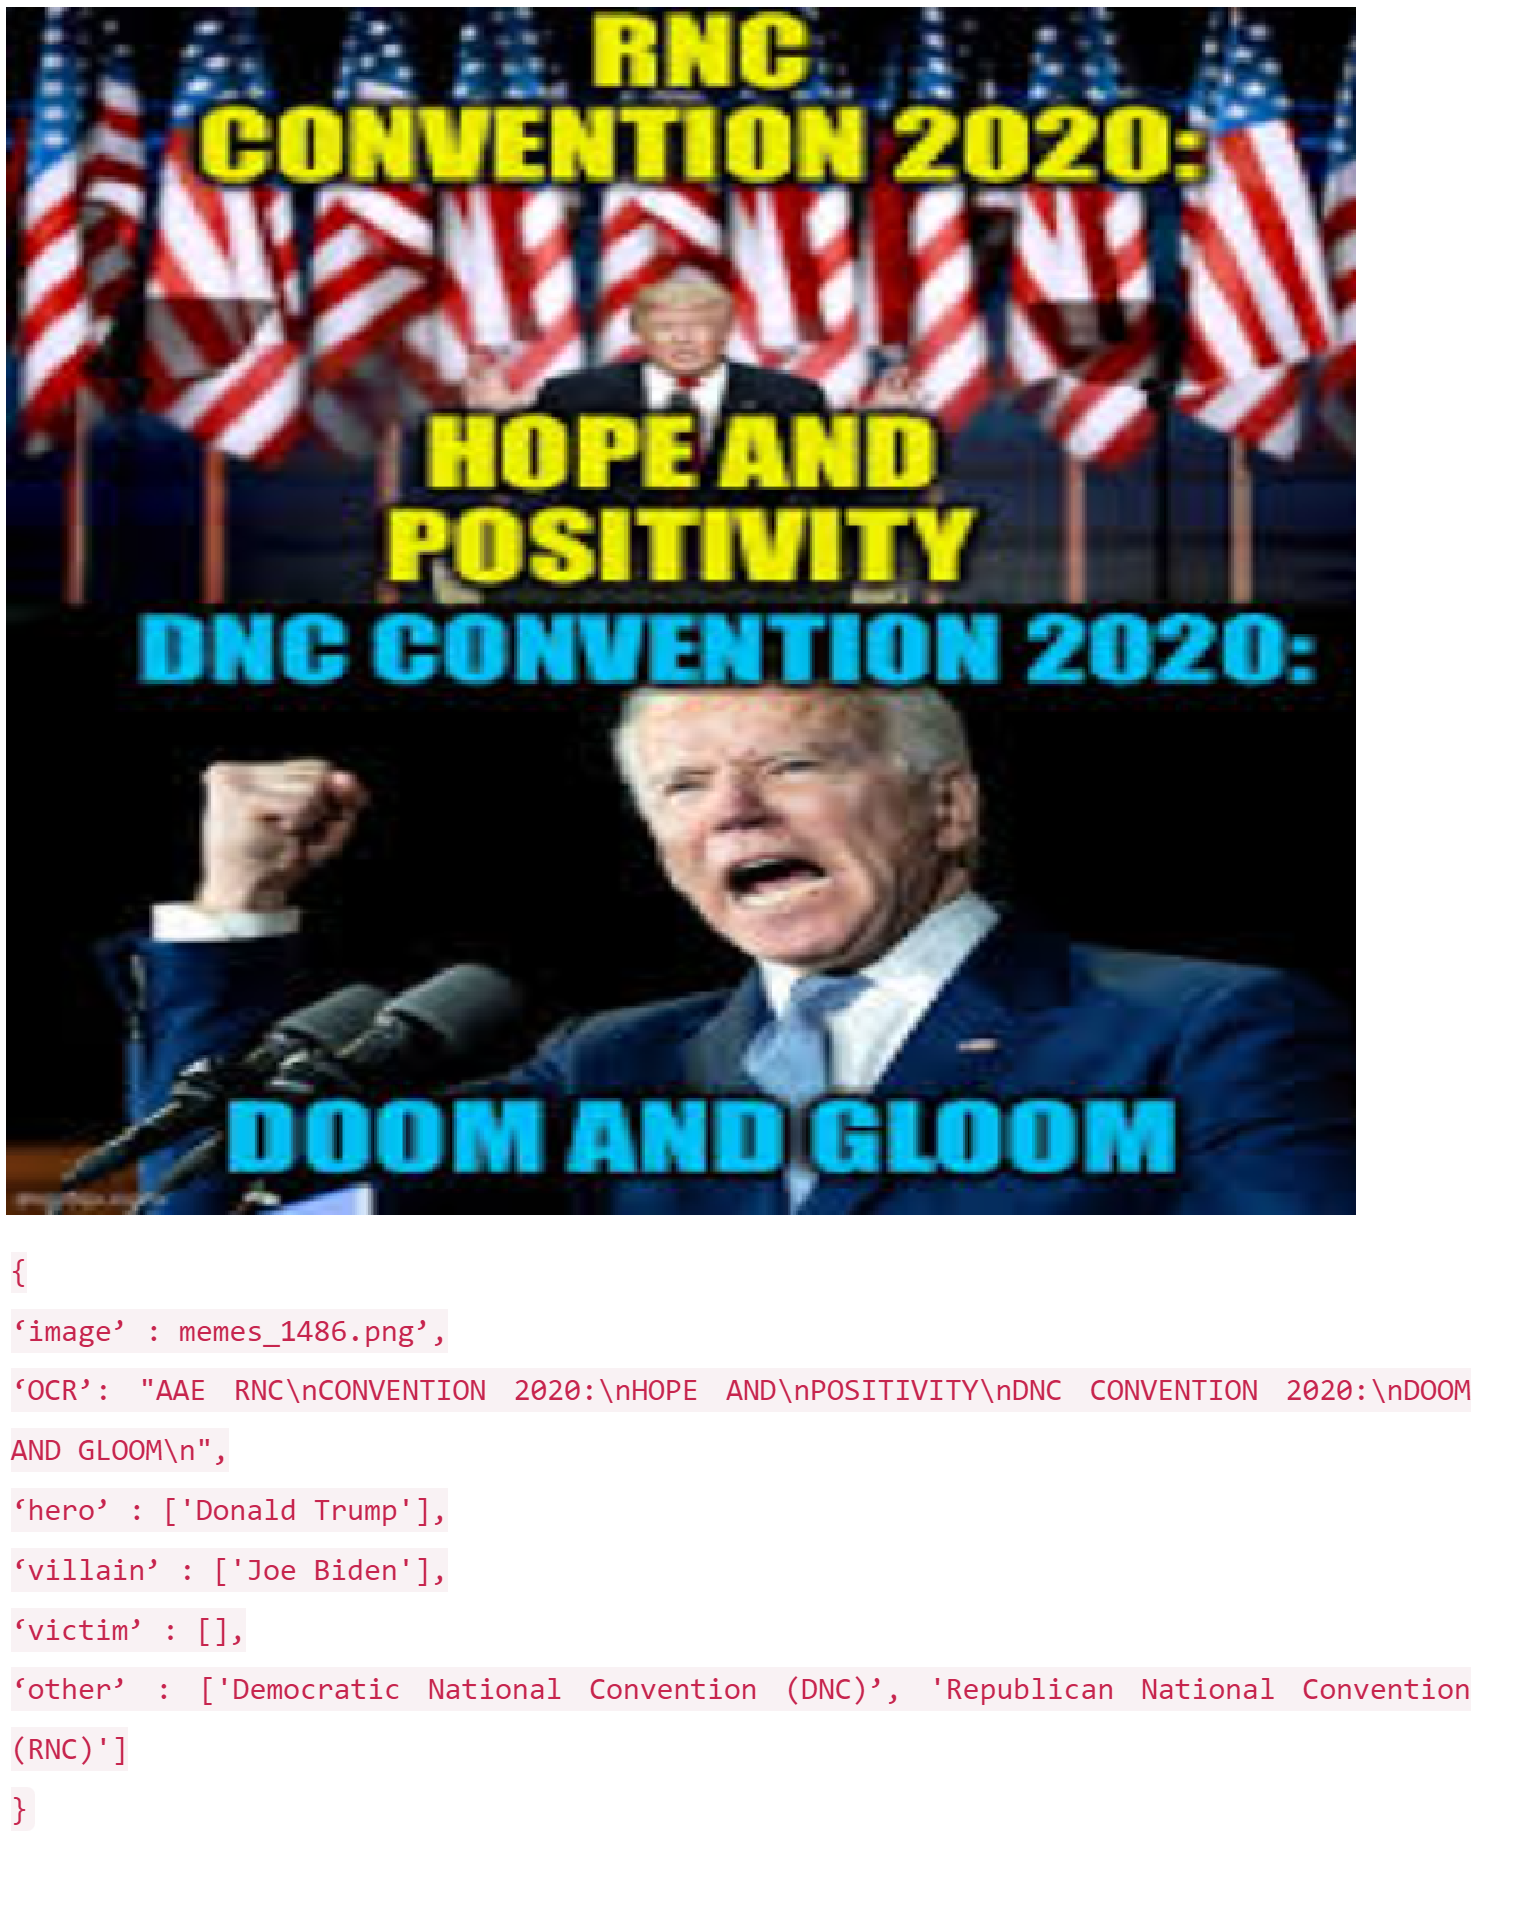
\includegraphics[scale=0.18 ]{examplememe2.png}
    \caption{CONSTRAINT dataset example}
    \label{fig:Constraint dataset examples}
\end{figure}

Depending on the textual information in the image, textual role classification is insufficient as some memes' underlying message requires understanding of the visual information it contains, especially with the use of humour and sarcasm often associated with the format.\\
The work done in this competition aims at finding unique and effective ways of tackling harmful meme classification as seen in the current social media space. An algorithm is designed for the task of role labelling for memes using a twin model (and ensemble) method. This Siamese network is constructed by combining the output of pre-trained State-of-the-Art (SoTA) models for both the visual components in the form of a CNN (Efficientnet-B7 \cite{tan2019efficientnet}) and for textual components using a transformer (DeBERTa \cite{he2020deberta}). The feature outputs obtained from both branches are then combined to obtain a final solution. Data analysis and investigation into potential bias in the dataset are also conducted to contextualise the task and present the difficulties of curating accurate multimodal datasets aimed at tackling the task for data in the wild \cite{gao2021logically}. 
In this paper, an overview of past work in the field is presented (section 2), followed by a deep dive into the problem statement as well as the method followed to respond to it (section 3), then data analysis (section 4). Experiments ran are presented in section 5, with results and discussion in section 6, and finally conclusion (section 7).


\section{Related Work}

There have been some work done with respect to semantic role labelling in text. The idea of ABSA(Aspect Based Sentiment Analysis) works along the same line. Hence, utilisation of DeBERTa has provided the SoTA results \cite{silvaaspect} due to the disentangled attention improving the focus more on the positional embeddings rather than just based on the word embeddings. Hence, improved results were also obtained in various SNLI task for this algorithm\cite{he2020deberta}.They are nowadays very popular in Natural Language Processing (NLP) as they usually get SoTA for a variety of NLP tasks such as classification, sentiment analysis, Named Entity Recognition, Translation, Question Answering, etc.
 

Classifying memes into relevant classes is a field that has got much more interest over the past few years. The Facebook Hateful meme competition\cite{kiela2020hateful} was a very publicised initiative to try and augment the field's capabilities. The task was a binary classification of hateful/not hateful meme based on a dataset curated by META. The winning solutions all comprised of ensembles of multimodal models. The Memotion competitions\cite{sharma2020semeval} are another example of work done in the meme space. This time, the classification was based on sentiment (positive, negative, neutral), as well as the strength of the sentiment and the underlying aim of the meme (satirical, humour or harmful). Multimodal models here also obtained the top scores.


Multimodal models have seen a change over the past few years from twin networks like Siamese  \cite{gu2018look} to models pretrained on multiple multimodal tasks such as image captioning and visual question answering using transformers \cite{devlin2018bert}. Object detection is used in these models to extract image features thanks to pre-trained two-staged detectors Faster R-CNN model \cite{ren2015faster}), or single-stage detectors (YOLO V3 \cite{adarsh2020yolo}). Inspired by BERT \cite{devlin2018bert}, models such as Uniter \cite{chen2019uniter} and VisualBERT \cite{li2019visualbert} use a transformer architecture to jointly encode text and images, while LXMERT \cite{tan2019lxmert} and ViLBERT \cite{lu2019vilbert} innovated by splitting their architectures in two, where a different transformer is applied to images and text individually before the features are combined by a third transformer. OSCAR (Object-Semantics Aligned Pre-training )(\cite{Li2020OscarOA}) add in the text input the class objects detected from the images by a Faster R-CNN detector called object tags. The use of object tags in images as anchor points, significantly ease the learning of alignments during the pretraining.
These models' effectiveness are demonstrated through their SoTA results on different multimodal dataset tasks such as NLVR2. This can be attributed to the models' increased capability to understand cross-modal correlations. However, these models are only as good as the data they've been pretrained on, which will present a challenge for the use case of the competition tackled in this paper. Another point is that the architectures of the textual streams of these models are a few years old (such as BERT) and inferior to the current SoTA (DeBERTa).
% add OSCAR?

\section{Methodology}

\subsection{Problem Statement}

The CONSTRAINT competition is a multimodal semantic role labelling multi-class classification problem. The aim is to classify the role of entities present in a meme using the image, its textual information and the entities it contains. The different classes are ("Hero", "Villain", "Victim", "Other"). The label applied for each entity depends on how the entity is presented in the meme:

Hero: The entity is glorified

Villain: the entity is vilified

Victim: the entity is victimised,

Other: none of the above.

\subsection{Ensembling :}
Our final model is an ensemble of 5 classifiers based on existing pretrained Unimodal (text) and Multimodal (text + images)  architectures. (see figure ~\ref{fig:final_model})
An ensemble combine several models to obtain a better generalised one. It usually gives a boost of performance in exchange for a more time-consuming model compared to more shallow model. Different methods of ensembling exist such as bagging, boosting, stacking, etc. We consider that this strategy will be very helpful to reduce the overfitting given the small number of instances we have, and how imbalanced the dataset is.
To combine our models, we average the predictions of our individual models.\\

%- empirical weighting based on the results of the individual models on the validation data

\begin{figure}
    \includegraphics[scale=0.3]{DeBERTa_Model.png}
    \caption{UniModal Model}
    \label{fig:UniModal}
\end{figure}

\begin{figure*}\centering
    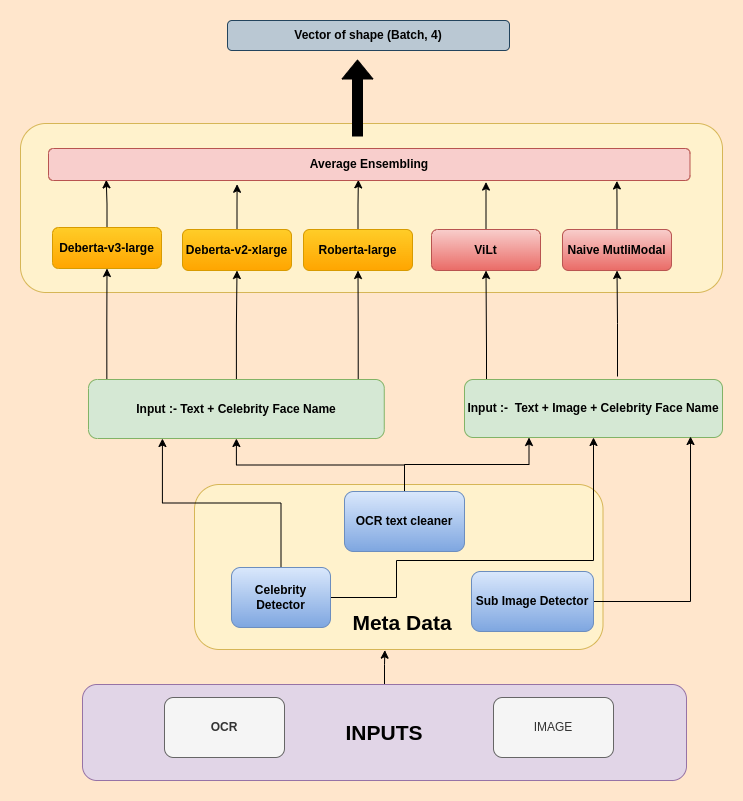
\includegraphics[scale=0.4]{diagram.png}
    \caption{Final model used for the Constraint22 competition.}
    \label{fig:final_model}
\end{figure*}
\subsubsection{Unimodal :}
We experimented a few unimodal architectures based on transformers  \cite{vaswani2017attention} such as DeBERTa  and RoBerta \cite{liu2019roberta} using only texts (OCR) and entities provided. The idea here was to see how much performance could be obtained just by textual information. These models are based on self-attention layers and an improved version of the BERT method pretrained on millions of sentences \cite{devlin2018bert} for language modelling. We fine-tuned on these models and found DeBERTa to be performing the best among the pre-trained BERT models. For the fine-tuning, the last FC layer added over pooler layer of DeBERTa. The last layer was a FC layer of size 4 to provide us with the respective role label. The architecture for this structure is given (see figure ~\ref{fig:UniModal}) . 
% (1) The first was a direct approach where we found the role for the entity based on the OCR provided. So Input would be " OCR Text + Entity ". The input of the transformer was as follows : "[CLS] Sentence OCR [SEP] entity to classify [SEP]"\\
% (2) The second approach consisted of incorporating image signals in the unimodal training. We ran the celebrity face detection algorithm and further added these faces names text with the extracted OCR.  The input of the transformer was as follow : "[CLS] Sentence OCR "\textbackslash n" face name [SEP] entity to classify [SEP]"\\
%(1) The first was a direct approach where we found the role for the entity based on the OCR extracted by the google model. So Input would be " OCR Text + Entity " and in output would be The input of the transformer for text data were then as follows : "[CLS] Sentence OCR [SEP] entity to classify [SEP]"\\
\subsubsection{Multi-Modal :}
We also experimented Multi Modal models which include as input data : images and texts (OCR + entity). 
We tried different approaches: \\
(1) The “Naive” approach consisted in extracting text features with a strong Language model - DeBERTa - and concatenating it with visual features with Convolutional Neural Network - EfficientNet-B7. We added on top of these concatenated features a Linear Layer to predict the class. \\
(2) The second approach was based on fine-tuning the whole image-text multimodal model. We experimented with two models: MMBT transformers ( Multimodal Bitransformers ) \cite{kiela2019supervised} and VisualBERT \cite{li2019visualbert} which has been pre-trained on classifying multimodal experiments.\\
(i) The MMBT transformer model utilise bert-base-uncased model as text encoder and the CLIP model \cite{https://doi.org/10.48550/arxiv.2103.00020} as image encoder. The main idea was to reuse the BERT text model we had fine-tuned for the task and freeze the 12 encoder layers. Further we fine-tuned the MMBT multimodal model by projecting the image embeddings to text token space. (ii) The VisualBERT was pretrained model \cite{li2019visualbert} for image-and-language tasks like VQA, VCR, NLVR2, and Flickr30Ks. We used the detectron2 embeddings \cite{ren2015faster} as image encodings with bert-base-uncased as text encoder to finetune the model. \\
(3) The last architecture used was ViLT \cite{kim2021vilt} (Vision and Language Transformers) which is one of the simplest architectures for a vision and language model.  ViLT is composed of a transformer module which extracts and processes textual and visual features without using separate embedder as it can be the case for MMBT for instance. That method gave a significant runtime and parameter optimisation. (see figure ~\ref{fig:multimodal})
%% Mention what is our best solution and what's it is composed of
\subsection{Meta Data extractions :}
We attempted to extract meta data information from images in order to improve the insight from those. Indeed, using only the OCR was sometimes insufficient because the entities were not always present in the text. Multiple strategies were investigated for gathering insights from images. 
\subsubsection{Celebrity Detector :}
(1) The most naive approach one we used, consisted in extracting text features with a strong Language model - DeBERTa - and concatenating it with visual features with Convolutional Neural Network - EfficientNet-B7. We added on top of these concatenated features a Linear Layer to predict the class. \\
(2) The second approach was based on fine-tuning the whole image-text multimodal model. We experimented with two models: MMBT transformers ( Multimodal Bitransformers ) \cite{kiela2019supervised} and VisualBERT \cite{li2019visualbert} which has been pre-trained on classifying multimodal experiments.\\
(i) The MMBT transformer model utilise bert-base-uncased model as text encoder and the CLIP model \cite{https://doi.org/10.48550/arxiv.2103.00020} as image encoder. The main idea was to reuse the BERT text model we had fine-tuned for the task and freeze the 12 encoder layers. Further we fine-tuned the MMBT multimodal model by projecting the image embeddings to text token space. (ii) The VisualBERT was pretrained model \cite{li2019visualbert} for image-and-language tasks like VQA, VCR, NLVR2, and Flickr30Ks. We used the detectron2 embeddings \cite{ren2015faster} as image encodings with bert-base-uncased as text encoder to finetune the model. \\
(3) The last architecture used was ViLT \cite{kim2021vilt} (Vision and Language Transformers) which is one of the simplest architectures for a vision and language model.  ViLT is composed of a transformer module which extracts and processes textual and visual features without using separate embedder as it can be the case for MMBT for instance. That method gave a significant runtime and parameter optimisation. (see figure ~\ref{fig:multimodal}) \href{https://github.com/Giphy/celeb-detection-oss}{Giphy's github}.

\subsubsection{Sub Image Detector}
The second observation made was that a MEME can contain multiples "sub images". In fact, as in the figure ~\ref{fig:example_meme_meta}, the MEME contains two images in it. A "sub images" detector was implemented based on YoloV5 (\href{https://github.com/ultralytics/yolov5}{https://github.com/ultralytics/yolov5}). We generated an artificial dataset, based on the Hateful MEME competition \cite{kiela2020hateful}, where we filtered and kept only the MEMEs with one image. Different single images were then combined to create one artificial MEME, with associated bounding boxes of the multiple subimages it contained. For the evaluation, 100 manually labelled images were used. The YOLO checkpoint is shared in our github solution. Our original idea was to extract with our detector each sub images from the MEME and associate each sentence of the OCR to the correct sub image with the name of the famous face if it existed. However, the OCR provided did not contain the coordinate of the sentence. We attempted to make the OCRed text match an open source OCR framework containing word coordinates, which yielded poor results. Therefore, the final multimodal model used the sub image as well as the face name into the text processing. The input of the transformer for text data was then as follows : "[CLS] Sentence OCR [SEP] entity to classify [SEP] face names [SEP]"
% explain sub image how model are trained
% face name extraction 
\begin{figure}
    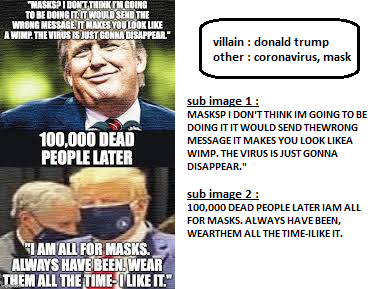
\includegraphics[scale=0.65]{covid_memes_151.png}
    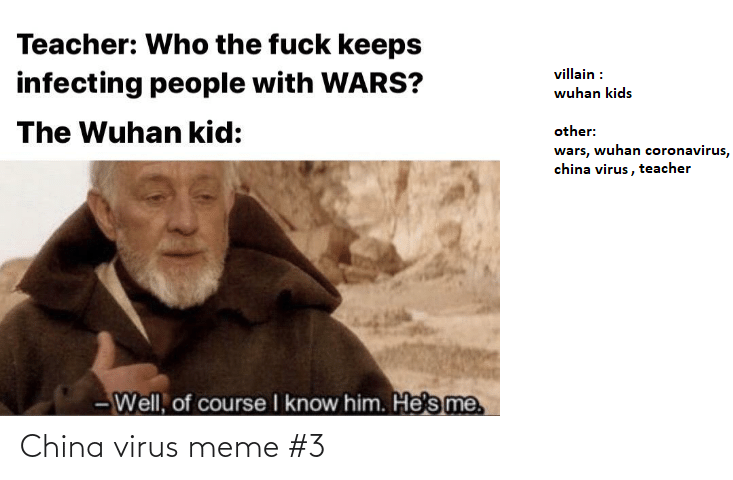
\includegraphics[scale=0.4]{covid_memes_4.png}
    \caption{Constraint dataset example : The first MEME contains two sub images whereas the second MEME don't have the entity we are looking for.}
    \label{fig:example_meme_meta}
\end{figure}

\section{Dataset}

The competition dataset consists of 2 memes subsets, one about US politics, and the other about Covid-19, totalling 5552 images with associated OCR and entity annotation in the training set, and 650 in the validation set. This size is very small to expect to build any robust SoTA vision or multimodal capabilities, training from scratch. 

The distributions of the 4 labels are heavily imbalanced (see table ~\ref{fig:distrib_class}). Over three quarters of the entities belong to the "other" class, and of the remaining classes, "villain" appears around twice as much as both the "hero" and "victim" class combined. An analysis of the entities in the dataset was undertaken and they were observed to be well balanced amongst the 4 classes. Indeed, as can be expected of using data from the political domain over the past few years, examples of common mentions were of "Donald Trump", "Barrack Obama", "The Republicans", "The Democrats". The fact that they were all amongst the most cited entities in each label indicates the sources used to curate the dataset was unbiased politically. Table  ~\ref{fig:top_entity} shows the top 5 most common entity per class.
\begin{table}
\begin{tabular}{ | c || c  || c || c || c |  }
 %\hline
 %\multicolumn{4}{|c|}{Country List} \\
 \hline
 \textbf{split} & \textbf{other} & \textbf{villain} & \textbf{hero} & \textbf{victim} \\
 \hline
 % (Counter({'other': 13702, 'villain': 2427, 'victim': 910, 'hero': 475}),
 %Counter({'villain': 305, 'other': 1589, 'victim': 121, 'hero': 54}))
 train  & 13702 & 2427 & 475 & 910\\ % 0.3998
  \hline
 train (ratio)  & 0.782 & 0.139 & 0.027 & 0.052\\ % 0.3998
  \hline
 val   & 1589 & 305 & 54 & 121\\ % 0.3998
  \hline
 val (ratio)  & 0.768 & 0.147 & 0.026 & 0.058\\ % 0.3998
 \hline
\end{tabular}
\caption{ distribution class of Constraint22 dataset}
 \label{fig:distrib_class}
\end{table}

\begin{table*}
\centering
\begin{tabular}{ | c || c || c || c || c |  }
 %\hline
 %\multicolumn{4}{|c|}{Country List} \\
 \hline
 \textbf{top-n entity} & \textbf{other} & \textbf{villain} & \textbf{hero} & \textbf{victim} \\
 \hline
 % (Counter({'other': 13702, 'villain': 2427, 'victim': 910, 'hero': 475}),
 %Counter({'villain': 305, 'other': 1589, 'victim': 121, 'hero': 54}))
 1  & donald trump & donald trump & donald trump & donald trump\\ % 0.3998
  \hline
 2   & coronavirus & joe biden  & barack obama & america\\ % 0.3998
  \hline
 3   & joe biden & democratic party & green party & people \\ % 0.3998
  \hline
 4   & barack obama & republican party & joe biden & barack obama\\ % 0.3998
  \hline
 5   & mask & barack obama & libertarian party & democratic party\\ % 0.3998
 \hline
\end{tabular}
\caption{ Top 5 most common entities per class in training dataset}
 \label{fig:top_entity}
\end{table*}

The OCRed text was obtained by running the Google OCR API on the images, which in some examples leads to imperfect text detection or extraction. These two issues materialise in the form of either poorly clustered text paragraphs into the appropriate text boxes, meaning sentences from two separate paragraphs would be concatenated together midway through, but also through more basic spelling mistakes.

Another point relevant to meme analysis is the presence of sub images inside each image. An image might itself contain two separate images which tell a different story, often contrasting between sentiments of entities in each, such as in figure ~\ref{fig:example_meme_meta}. 

A big challenge with this task of entity classification is detecting where the entity is mentioned whether in the OCR or in the image. Table 3 shows the percentage of entities present in the OCR of the image in the dataset. Some examples, such as in figure ~\ref{fig:example_meme_meta}, have one of the entities to classify not present in neither the OCR nor the image, and must be classified from understanding of context, which makes the task more difficult.

\begin{table} 
\centering
\begin{tabular}{ |c||c|  }
 \hline
 \textbf{split} & \textbf{ratio matching} \\multimodal
 \hline
train  & 0.572\\ % 0.3998
\hline
val  & 0.602\\ % 0.3998
 \hline
\end{tabular}
\caption{ Ratio of entities which are present in OCR provided}
 \label{fig:ratio_entity}
\end{table}

\section{Experiments}
\subsection{Experimental Setting : }
To train and evaluate our different models, we used the Google Cloud Service with VM using the V100 GPU (16GB) and A100(40GB). We use the famous Pytorch framework with the Huggingface library in python. All our training used mixed precision and gradient accumulation in order to speed up some training time and allow larger model training.
\subsection{Data Analysis :}
Data Analysis was performed in order to understand the underlying problem better and find potential imbalances that could be leveraged for higher performances. The distribution of the number of entities per class, as well as each individual entity for each class was computed. Based on an a given entity, the aim was to try and predict which class it would most likely belong. An issue we came across was that some entities were mentioned in different ways: "americans" vs "american people". A rule-based approach was incorporated in an attempt to group these similar terms together. 

Analysis was running on the OCR as well as the output of the celebrity detection model to determine if the entity was mentioned inside the text, in the image, both or neither. References to single entities in the textual format would vary, one example being for the entity "Donald Trump", which would be referenced as "Trump", "donald", "Donald Trump" to name a few. A rule based classifier was implemented to group these terms together for the entities that showed up most frequently.

A prediction was made based on the heuristics of the imbalances found to establish a baseline model, by classifying all the entities as "other", which is the class which contains over 75\% of entities. Learning models would have to beat the accuracy of this rule based baseline to add value.

\subsection{Augmentations :}
Only one augmentation was used during the training. The augmentation was applied to the entity which needed to be classified. In fact, the entities provided were all without any punctuation and in lowercase format. We created a simple script which found the entity in the original text. The original text could contain punctuation and/or uppercase letter. We used this augmentation for the training, not the inference of the test set.
\subsection{Unimodal NLP : }

%% TO CORRECT 
We trained a few competitive transformer architectures on text-only data, DeBERTa-v3 and RoBERTa.\subsubsection{DeBERTa}
Two experiements were conducted for DeBERTa
(1) The first was a direct approach where we found the role for the entity based on the OCR extracted by the google model. The input of the transformer was as follows : "[CLS] Sentence OCR [SEP] entity to classify [SEP]"\\
(2) The second approach consisted of incorporating image signals in the unimodal training. We ran the celebrity face detection algorithm and further added these faces names text with the extracted OCR.  The input of the transformer was as follow : "[CLS] Sentence OCR "\textbackslash n" face name [SEP] entity to classify [SEP]"\\
We utilized both DeBERTa-small and DeBERTa-large for these experiments.
During the training, a batch size of 16 was used, with a sequence length of 128  and a linear scheduler where the learning rate was reduced linearly during the training. The initial learning rate was $1e-5$, gradient accumulation is set at 3 epochs, and the optimizer used was AdamW. We trained these models for 6-7 epochs.
\subsubsection{RoBERTa large}
A batch size of 8 was used, with a sequence length of 275 and a linear scheduler where the learning rate was reduced linearly during the training. The initial learning rate was $5e-6$, and the optimizer used was AdamW. We trained these models for 6-7 epochs.
\subsection{MultiModal}
\subsubsection{Naive Merging:}
We used a batch size of 4 (A100 GPU), with a sequence length of 275. As a unimodal model, we use the face name in the text input processing. We use 4 sub images when they exist and the MEME image. We use an attention system inspired by the Word Attention in \cite{li2019bidirectional} , before concatenating the image features with the text features. We use a linear scheduler where the learning rate is reduced linearly during the training. The initial learning rate is $5e-6$, gradient accumulation is set at 3 epochs, and the optimizer used is AdamW. We trained these models for 7-8 epochs with early stopping of 2 epoch.
\subsubsection{ViLT:}
We use a batch size of 4, with a sequence length of 275. As unimodal model, we use the face name in the text input processing. We don't use here a linear scheduler, but ReduceLROnPlateau where the learning rate is reduced by a factor of 0.5 when there is no improvement during  5 epochs. The initial learning rate is $2e-5$, and the optimizer used is Adam. We trained these models for 7-8 epochs with early stopping of 2 epoch.

\subsubsection{MultiModal : MMBT and VisualBERT}
We use a batch size of 16, with a sequence length of 128. As for multimodal model, we use the image embeddings obtained from CLIP\cite{radford2021learning} and detectron2 \cite{ren2015faster} model individually for MMBT and VisualBERT. The text model used in both the architecture is bert.  We use a linear scheduler where the learning rate is reduced linearly during the training. The initial learning rate is $1e-5$, gradient accumulation is set at 3 epochs, and the optimizer used is AdamW. We trained these models for 7-8 epochs with early stopping of 2 epoch.
\subsection{Ensembling :}
To improve the robustness of our solution we decide to combine 5 of our models (table ~\ref{fig:results}). We chose the models to combine based on the results of the validation score and also the diversity they could bring. For instance, we did not select DeBERTa-v3-small because it is just a smaller version of DeBERTa-v3-large. We select only two multimodal models, as most of them perform quite badly compared to the unimodal. Otherwise they would just harm the ensemble.

\begin{table*}
\centering
\begin{tabular}{ |p{8cm}||c||c| }
 \hline
 \textbf{Model} & \textbf{F1-score val (macro)} & \textbf{F1-score test (macro)} \\
 \hline
 (a) DeBERTa-v2-xlarge w/o face's name  & 0.54 & 0.53  \\  
 \hline
 (b) DeBERTa-v3-small w/o face's name  & 0.46 & 0.46  \\  
  \hline
 (c) DeBERTa-v3-small w face's name  & 0.48 & 0.47  \\  
  \hline
 (e) DeBERTa-v3-large w/o face's name  & 0.55 & 0.55  \\  
 %  \hline
 %(5) DeBERTa-v3-large w/ face's name, 275 seq length  & 0.53 & 0.56  \\  
  \hline
 (f) DeBERTa-v3-large w/ face's name  & 0.56 & 0.57  \\  
  \hline
 (g) RoBERTa-large w/ face's name  & 0.53 & 0.51  \\  
 \hline
  \hline
  (h) ViLT w face's name  & 0.42 & 0.42  \\  
  \hline
 (i) Naive Multi Modal (DeBERTa-v3-large + EfficientNetB7) w/ face's name  & 0.525 & 0.55  \\
  \hline
 (j) MMBT (BERT + CLIP) w/ face's name  & 0.48 & 0.46  \\  
  \hline
 (k) VisualBERT w/ face's name  & 0.43 & 0.44  \\  
  \hline
 Ensembling Mean(a, f, g, h, i)  & \textbf{0.578} & \textbf{0.583}  \\  
  \hline
\end{tabular}
\caption{Experiments Results}
 \label{fig:results}
\end{table*}


\section{Results and discussion}
% Our best unimodal results were based on DeBERTa-v3-large with the Huggingface library in python.\\
Just the simple experiment classifying all entities as "other" yielded 0.21 f1 score. We experimented with various models starting with just the text-based model, further adding image signals to using the image embeddings and finally a fully image-and-language based multimodal model to evaluate the model architecture efficiency in predicting a low resource multimodal problem. Here are some observations :-\\
(1) Unimodal - We can see the difference in results moving from "DeBERTa-v3-small" to "DeBERTa-v3-large" in Table ~\ref{fig:results}. We can also see 2\% improvement in the model when we tried to add image signal naively by adding the celebrity face name in text. \\
(2) Multi-Modal -  We can see that multimodal model under performed a lot as seen in  Table ~\ref{fig:results}.  We tried to fine-tune the Visual-BERT model and the mmbt model i.e. pre-trained vision-and-language model but they seem to under perform due to the lack of pre-training data. As they had been pre-trained on much less data and very different problem like VQA , it failed to capture the model understanding required for the transfer learning. So as to solve this issue we went ahead and utilised trained "DeBERTa-v3-large" model final output layer embeddings and concatenated them with pooled sub-image embedding with EfficientNetB7. Thus we utilised the transfer learning from both the models to give us the optimum results.\\
(3) Ensemble - The ensemble approach was our final approach where we combined all the different model outputs . We tried various ensembles and blending techniques but we got the best LB score with averaging of ViLT, RoBERTa large, DeBERTa large, naive multimodal and DeBERTa-xlarge models.
Final test set results and competition leaderboard are presented in Table \ref{tab:factify_leaderboard}. Our best model ("Ensemble") outperforms all competition systems and best baseline models. Test result of $Ensemble$ model achieved 0.58 avg. F1.

% \cite{factifyreview}
% Weighted average F1 scores for 5-way classification for our SemEval 2013 task 7 submissions, along with the maximum and mean performance



\begin{table} 
\centering
\begin{tabular}{ |c||c||c|    }
 \hline
 \textbf{Rank} & \textbf{Team}  & \textbf{Final accuracy}\\
 \hline
 1 & Logically & \textbf{58.671\%} \\
 \hline
2 & {c1pher}       & 55.240\% \\
\hline
3 & {zhouziming} & 54.707\% \\
\hline
4 & {smontariol} & 48.483\% \\
\hline
5 & {zjl123001} & 46.177\% \\
\hline
6 & {amanpriyanshu}& 31.943\% \\
\hline
7 & {fharookshaik} & 23.855\% \\
\hline
8 & {rabindra.nath} & 23.717\% \\
 \hline
\end{tabular}
\caption{Constraint22 Leaderboard}
 \label{tab:factify_leaderboard}
\end{table}

\section{Conclusion}
\label{sec:bibtex}
We described our participation in the CONSTRAINT 2022 Shared Task on "Detecting the Hero, the Villain, and the Victim in Memes" with the implementation of various models. Ensemble model based system outperforms all the models on val set and test set. A challenge in this task is the low resource of data available for training models. Hence, transfer learning provides the best results.\\
The best performing model in this competition combines the simple averaging of ViLT, RoBERTa large, DeBERTa large, naive multimodal and DeBERTa xlarge models. The ensemble seems to perform the best as the data size is small and we  use a large model to allow for better transfer learning, This ultimately leads to some overfit of models but applying the averaging improves the results, like the boosted trees systems. \\

We found that there were two major challenges with the problem :- (i) The entities were sometimes not present in the image or the text. (ii) The size of data required to learn this implicit learning was not sufficient. This  ultimately undermines the performance of our deep learning architecture.\\ Creating a dataset for real-word multimodal problems, particularly the natural language inference problem of role labelling is challenging \cite{le2020adversarial}. We appreciate the work by the CONSTRAINT 2022 organizers, yet, a more elaborate and extensive data would make this dataset more suitable for benchmarking. As an emergent research field, we hope our extensive model analysis and proposed solutions can act as baseline and inspire further work.

% More effort is required to tackle
% the dataset gathering challenge of minimising biases from human annotators which would make the dataset better reflecting real-world challenges. As an emergent research field, we hope our extensive model
% analysis and proposed solutions can act as baseline and inspire further work.


% Entries for the entire Anthology, followed by custom entries
\bibliography{anthology,custom}
\bibliographystyle{acl_natbib}

\newpage

\appendix
\newpage
\begin{figure*}
\section{Appendix I}
    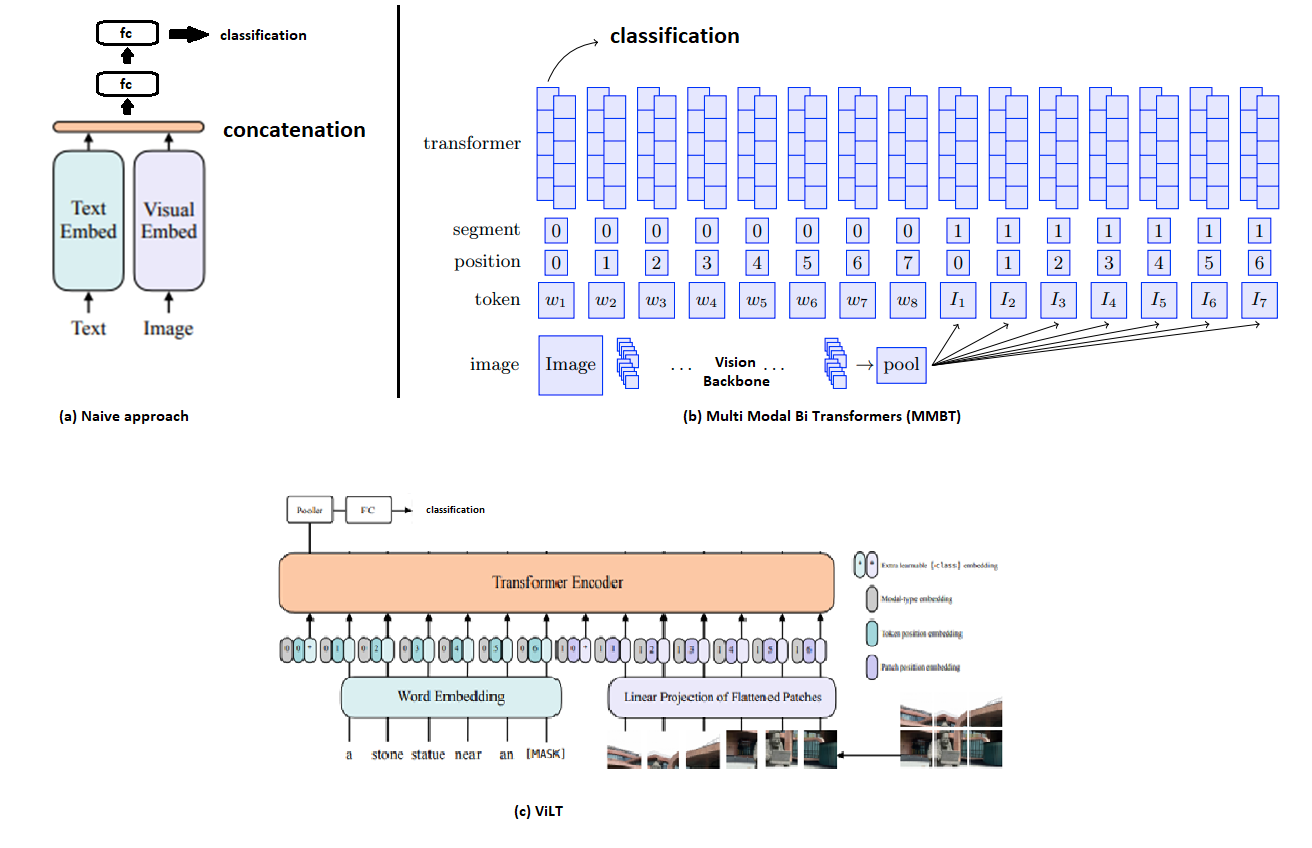
\includegraphics[scale=0.5]{MultiModal.png}
    \caption{Example of Multimodal Architecture used}
    \label{fig:multimodal}
\end{figure*}
\label{sec:appendix}

\end{document}
